\section{Speculation Buffer} \label{Speculation Buffer}

The side-channel which forms the basis of multiple Spectre variants is the modification of data cache state during speculative execution.
To improve performance, modern out-of-order cores will speculatively fetch data into the core on a load miss.
However, in the event that the load miss is misspeculated, the refill data is still written into the cache, potentially evicting other resident cache lines.
As seen in the attack variants described earlier, by carefully measuring the execution times of repeated loads, attacker code can inspect the state of the cache and infer the destination addresses of misspeculated loads by the victim code.

To address this issue, the tag and data arrays must be considered as part of the ``architectural state'' of the machine, since their contents will affect the ``architectural'' results of timing measurements performed by attacker code.
Similar to how architectural register state is managed in the execution pipelines of out-of-order machines, a secure core must only allow correctly speculated, committing instructions to modify the cache state.
A proposed approach is to hold speculated load data in an ``L0 Speculation buffer'' that can be flushed when misspeculation is detected.
This prevents misspeculated loads from affecting the state of the cache, while still allowing correctly speculated loads to broadcast their data into the rest of the machine as soon as possible, maintaining performance. If well implemented, such a buffer could slightly improve performance by deferring the eviction of prior contents, slightly reducing the miss latency, and could even be combined with a store coalescing buffer - another useful ``L0 buffer'' structure.

\subsection{Boom's Data Cache}
BOOM is currently configured with RocketChip's non-blocking L1 cache. This cache is single-ported and intended for use with the in-order Rocket core: a consequence is that the cache lacks the concept of speculation. Boom's pipeline expects the ability to kill any misspeculated operations the cycle after misspeculation is detected. Therefore a data cache ``shim'' structure is used to track operations inside the datacache, killing them if they were found to be misspeculated. To implement our speculaton buffer, we needed to pass both per-request and global speculatative metadata.

\subsection{Miss Status Holding Registers}
We implement a speculation buffer, which we have named SpecBuf, as part of the Miss Status Holding Registers (MSHRs) in BOOM's L1 data cache. The MSHRs hold the status of inflight memory requests made by the L1 cache to the L2 memory bus.
In the original data cache, L2 cache refills would write the refill data into the tag and data arrays before waking up the corresponding MSHRs to return the load data to the core.
To implement SpecBuf, we modified cache refills to instead write the refill data into per-MSHR cache line buffers.

On misspeculation, the misspeculated MSHR entry is flushed along with any load data that has been returned. Only after the load which allocated the MSHR entry is known to be committed is the evicted cache line written back (if dirty) and the new cache line written into the tag and data arrays. This effectively prevents misspeculated loads from altering the state of the cache.

Since speculating past loads is necessary for performance, we allow bypassing refill data out of the SpecBuf, before the data is committed. The consequence of this bypassing is that the service time for a cache miss is slightly reduced compared to the original behavior; data can be forwarded out prior to the updating of the cache meta data. On the flipside, the total MSHR allocation time is longer than in the original behavior.

Another subtlety of the MSHRs is the per-MSHR replay queues, which hold subsequent requests to the same cache-line. These queues are necessary for handling consecutive (secondary) load misses to the same cache line while the initial (primary) miss is being handled. Following the acquisition of the requested cache line, our SpecBuf will eagerly empty the replay queues until a store miss is seen in the queue. Since stores issued to the memory system are always non-speculative, the cache line can be immediately committed at this point.

\begin{figure}[h]
  \begin{center}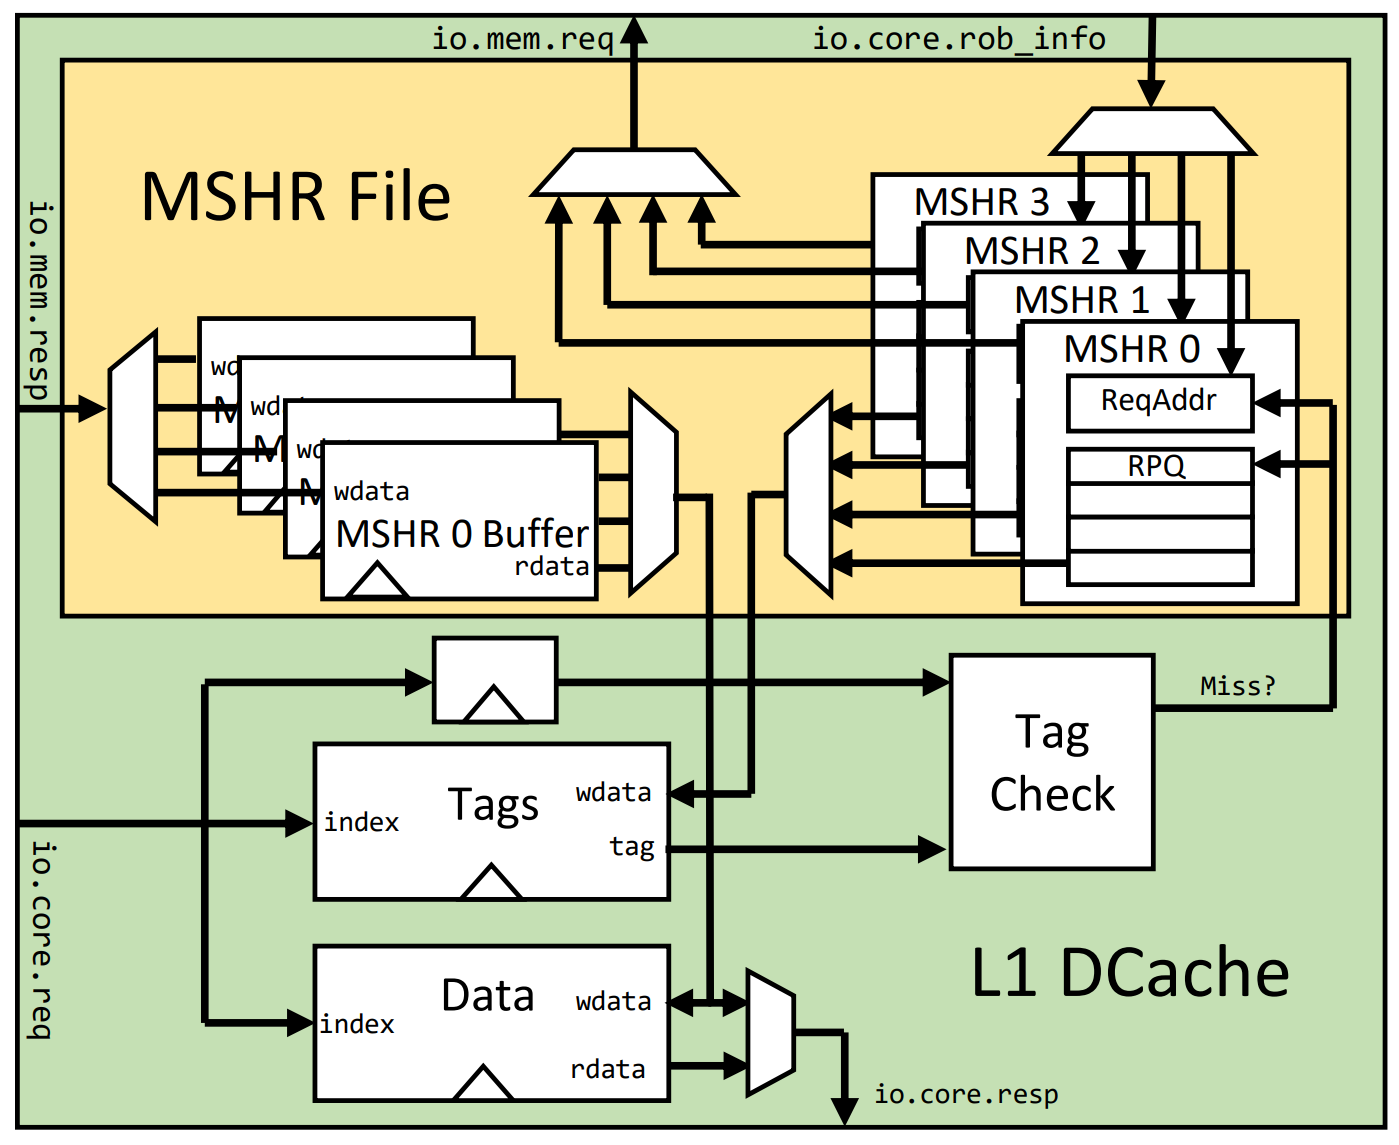
\includegraphics[scale=0.17]{dcache.png}\end{center}
  \caption{Overview of modified L1 data cache}
\end{figure}

\subsection{Point of No Return}
In the base implementation of the speculation buffer, entries in the buffer are only deallocated when the instruction is reached by the head of the reorder buffer (ROB). However, this can result in heavy MSHR utilization, as many instructions may reside between a waiting load and the commit head. However, we observe that many of those instructions, while still inflight, can be marked as guaranteed to commit.

This informs the concept of a ``point-of-no-return'' (PNR) in the ROB, in addition to the commit head. While the commit head tracks the next instruction which will commit the architectural state, the PNR tracks instructions which are guaranteed to eventually commit, even if they have not yet completed execution. In other words, the PNR points at the oldest instruction which may cause misspeculated execution; an unsafe instruction, such as a branch which has not yet executed. If an instruction is marked as safe, the PNR will pass it whether or not it has completed executing. We observe that refills in the spec-buffer can be committed to the cache as soon as the PNR passes the instruction which triggered them. This reduces pressure on MSHR resources and prevents backpressure on incoming cache requests.

To reduce the performance impacts of SpecBuf, we implemented a PNR in the ROB. Two versions were implemented. The first ``simple-PNR'' will only mark at most one ROB row per cycle as ``guaranteed to commit''. We also implemented a more complex ``fast-PNR'' that can mark an arbitrary number of rows per cycle, essentially ``jumping over'' groups of safe instructions to the oldest unsafe instruction. These are illustrated in figure~\ref{PNR}: the position of the PNR pointer on the subsequent cycle is shown for both the simple and fast versions.

\begin{figure}[h]
  \begin{center}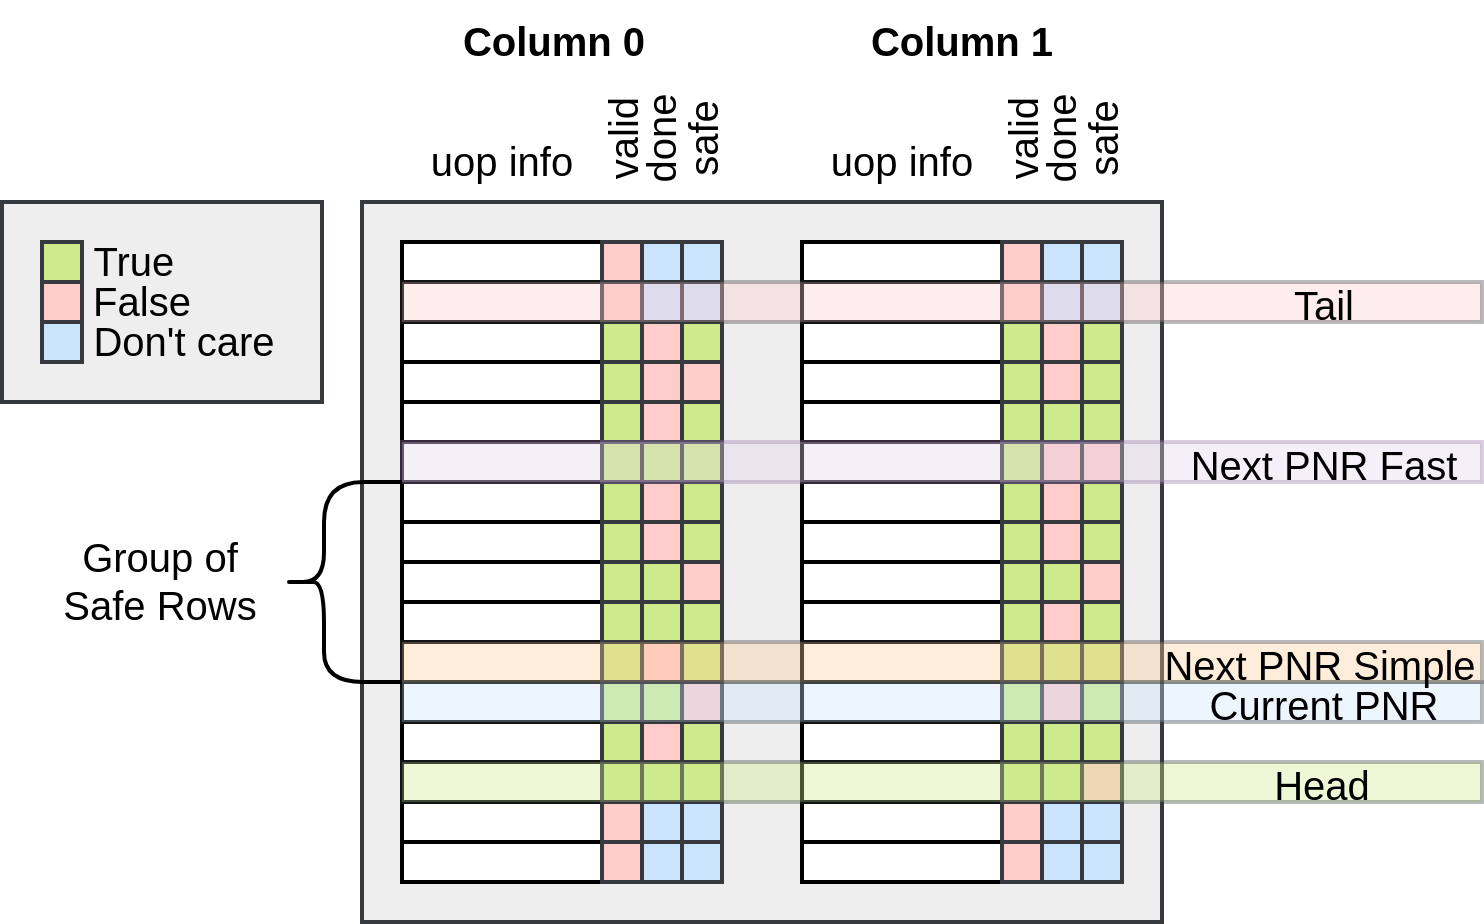
\includegraphics[scale=0.17]{rob_pnr.png}\end{center}
  \caption{Overview of PNR in ROB}
  \label{PNR}
\end{figure}

\subsection{Physical Optimization}
The speculative cache line buffers are by far the most physically costly addition to our secure boom variant. These buffers do not often need to be accessed simultaneously, and thus can be ``factored out'' of the MSHRs and into a single ported (1RW) or dual ported (1R/1W) SRAM. This would significantly decrease the (already modest \ref{syn}) area overhead incurred by these cache line buffers compared to when they are synthesized out of flip-flops.

\subsection{MSHR File as a Sidechannel}
A limitation which affects our current MSHR file implementation is that MSHRs are not always immediately deallocated after being killed. This limitation opens up several potential sidechannels which Spectre style attacks could use to extract information. For instance, when combined with the limitation of only allowing a single inflight miss to a particular cache set, the following attack surfaces: an attacker could perform their malicious call on a victim function repeatedly, following each call immediately with a single load which is known to miss, rather than an inspection of an entire attack array. If one of these loads took longer than expected of a miss, the attacker could deduce that a killed miss to the same set was being held by the MSHR, waiting for a response from the data bus. From this, the attacker infers part of the address used in the victim's secret-dependent load; 6 bits in a cache with 64 sets. This attack may be more difficult to perform than the standard attack, as there is a limited time window the MSHR will remain allocated following being killed. Additionally, this attack would be far slower as the victim call and probing sequence needs to be performed an average of $num\_sets/2$ times to read out $log_{2}(num\_sets)$ bits.

\subsubsection{Fully Associative MSHR File}
Making the MSHR file fully associative would aid in mitigating the side channel mentioned above. The number of MSHRs allocated could still be used as a side channel, however. The reason we have not made the MSHR file fully associative is the random replacement policy employed by the Rocket cache, which assumes only a single miss may be inflight per cache set. We would need to augment this policy with an index associative structure, with as many entries as there are MSHRs. This structure would track which ways of a particular set are scheduled to be replaced by an inflight miss. Note that this would not entirely mitigate the side channel, as the number of inflight misses to a particular set is now limited by the number of ways, as opposed to being singular. Thus, the attacker would need to simply perform more accesses.

\subsubsection{Immediately Killable MSHRs}
MSHRs are not immediately killable because they must acknowledge the L2 data bus when it has returned with the refill data. They must additionally forward out speculative loads which will be received and killed by the data cache shim; failure to forward out loads will result in a resource leak in this structure. To implement this functionality, we would need to implement a structure which tracks inflight refill requests. This structure would need to have more entries than the number of MSHRs; free entries would be mapped onto MSHRs upon a primary cache miss. Upon receiving a bus response, they would ``wake up'' their corresponding MSHR. Entries would be disassociated from MSHRs if the MSHR was killed early, and would be deallocated upon receiving and acknowledging their bus response. Additionally, we would be required to forward ``phony'' load responses to the data cache shim.
